\documentclass[thesis.tex]{subfiles}

\begin{document}
\chapter{Results}
\section{Proof of concept}
This section can be seen as an introduction to the usage of the tool in Appendix \ref{ref:tool} as much as it is a display of results. Even though this thesis is mainly concerned with the conceptual algorithm and not the implemented tool, every test case starts with the commands which is run to produce the graphical output. This is mainly done to clearly show the input data going in to the experiments, but also as introductionary examples to users of the tool. 
\par\noindent
We start out by building a graph from a single sequence:\\
\begin{figure}[H]
  \begin{mdframed}
    \includegraphics[width=\textwidth]{outputs/equal-merge.png}
  \end{mdframed}
  \caption{A reference graph made from the sequence ``ACGTATTAC''}
  \label{fig:output_ref}
\end{figure}
\subsection{Equal sequences}
\begin{figure}[H]
  \begin{subfigure}[t]{\textwidth}
    \begin{mdframed}
      \includegraphics[width=\textwidth]{outputs/equal-alignment.png}
    \end{mdframed}
    \subcaption{}
  \end{subfigure}
  \begin{subfigure}[t]{\textwidth}
    \begin{mdframed}
      \includegraphics[width=\textwidth]{outputs/equal-merge.png}
    \end{mdframed}
    \subcaption{}
  \end{subfigure}
  \caption{The result of aligning (a) and merging (b) the sequence ``ACGTATTAC'' against the reference graph seen in Fig. \ref{fig:output_ref}}
  \label{fig:output_equal}
\end{figure}
\subsection{SNPs}
\begin{figure}[H]
  \begin{subfigure}[t]{\textwidth}
    \begin{mdframed}
      \includegraphics[width=\textwidth]{outputs/snp-no-margin-alignment.png}
    \end{mdframed}
    \subcaption{}
  \end{subfigure}
  \begin{subfigure}[t]{\textwidth}
    \begin{mdframed}
      \includegraphics[width=\textwidth]{outputs/snp-no-margin-merge.png}
    \end{mdframed}
    \subcaption{}
  \end{subfigure}
 \caption{The result of aligning (a) and merging (b) the sequence ``ACGGATTAC'' against the reference graph seen in Fig. \ref{fig:output_ref} with $\lambda=0$}
\end{figure}
\begin{figure}[H]
  \begin{subfigure}[t]{\textwidth}
    \begin{mdframed}
      \includegraphics[width=\textwidth]{outputs/snp-alignment.png}
    \end{mdframed}
    \subcaption{}
  \end{subfigure}
  \begin{subfigure}[t]{\textwidth}
    \begin{mdframed}
      \includegraphics[width=\textwidth]{outputs/snp-merge.png}
    \end{mdframed}
    \subcaption{}
  \end{subfigure}
  \begin{subfigure}[t]{\textwidth}
    \begin{mdframed}
      \includegraphics[width=\textwidth]{outputs/snp-merge-two.png}
    \end{mdframed}
    \subcaption{}
  \end{subfigure}
  \caption{The result of aligning (a) and merging (b) the sequence ``ACGGATTAC'' against the reference graph seen in Fig. \ref{fig:output_ref} and then merging the sequence ``ACGCATTAC'' (c) with $\lambda=1$}
  \label{fig:output_snp}
\end{figure}
\subsection{Indels}
\begin{figure}[H]
  \begin{subfigure}[t]{\textwidth}
    \begin{mdframed}
      \includegraphics[width=\textwidth]{outputs/insertion-alignment.png}
    \end{mdframed}
    \subcaption{}
  \end{subfigure}
  \begin{subfigure}[t]{\textwidth}
    \begin{mdframed}
      \includegraphics[width=\textwidth]{outputs/insertion-merge.png}
    \end{mdframed}
    \subcaption{}
  \end{subfigure}
  \caption{The result of aligning (a) and merging (b) the sequence ``ACGTAATTAC'' against the reference graph seen in Fig. \ref{fig:output_ref}}
  \label{fig:output_insertion}
\end{figure}
\begin{figure}[H]
  \begin{subfigure}[t]{\textwidth}
    \begin{mdframed}
      \includegraphics[width=\textwidth]{outputs/deletion-alignment.png}
    \end{mdframed}
    \subcaption{}
  \end{subfigure}
  \begin{subfigure}[t]{\textwidth}
    \begin{mdframed}
      \includegraphics[width=\textwidth]{outputs/deletion-merge.png}
    \end{mdframed}
    \subcaption{}
  \end{subfigure}
  \caption{The result of aligning (a) and merging (b) the sequence ``ACGTTTAC'' against the reference graph seen in Fig. \ref{fig:output_ref}}
  \label{fig:output_deletion}
\end{figure}[H]
\subsection{Structural variations}
\clearpage
\section{Efficiency}
\subsection{Building the index}
\begin{figure}
    \begin{tikzpicture}
      \begin{axis}[scale only axis,height=\textwidth,width=\textwidth,xmin=0,ymin=0,xmax=152451,ymax=122654330941,scaled ticks=false, xlabel={Number of vertices}, ylabel={Nanoseconds (ns)}]
        \addplot[color=black,mark=*] coordinates {
          (701,597127494)
          (3416,2050636347)
          (20931,13858701254)
          (37801,25401423058)
          (100351,77928851412)
          (152451,122654330941)
        };
      \end{axis}
    \end{tikzpicture}
    \caption{Runtime for the build index procedure}
\end{figure}
\begin{figure}
  \begin{subfigure}[t]{0.4\textwidth}
    \begin{tikzpicture}[trim axis left]
      \begin{axis}[scale only axis,height=\textwidth,width=\textwidth,xmin=0,ymin=0,xmax=152451,ymax=122654330941,scaled ticks=false]
        \addplot coordinates {
          (701,9404263)
          (3416,51489024)
          (20931,623903806)
          (37801,1031820116)
          (100351,5487825644)
          (152451,11328920839)
        };
      \end{axis}
    \end{tikzpicture}
    \subcaption{Time used building the graph}
  \end{subfigure}
  \hfill
  \begin{subfigure}[t]{0.4\textwidth}
    \begin{tikzpicture}[trim axis left]
      \begin{axis}[scale only axis,height=\textwidth,width=\textwidth,xmin=0,ymin=0,xmax=152451,ymax=122654330941,scaled ticks=false]
        \addplot[color=green,mark=*] coordinates {
          (701,65184733)
          (3416,138556745)
          (20931,269431681)
          (37801,2788165703)
          (100351,6905517064)
          (152451,10007919085)
        };
      \end{axis}
    \end{tikzpicture}
    \subcaption{Time used building the index}
  \end{subfigure}
  \begin{subfigure}[b]{0.4\textwidth}
    \begin{tikzpicture}[trim axis left]
      \begin{axis}[scale only axis,height=\textwidth,width=\textwidth,xmin=0,ymin=0,xmax=152451,ymax=122654330941,scaled ticks=false]
        \addplot[color=red,mark=*] coordinates {
          (701,522174790)
          (3416,1860265733)
          (20931,1296505592)
          (37801,21581107294)
          (100351,65535179527)
          (152451,101317180800)
        };
      \end{axis}
    \end{tikzpicture}
    \subcaption{Time used writing the index\vspace{\baselineskip}}
  \end{subfigure}
  \hfill
  \begin{subfigure}[b]{0.4\textwidth}
  \begin{tikzpicture}[trim axis left]
    \begin{axis}[scale only axis,height=\textwidth,width=\textwidth,xmin=0,ymin=0,xmax=152451,ymax=122654330941,scaled ticks=false]
      \addplot[name path=axis] coordinates {
        (0, 0)
        (152451, 0)
      };
      \addplot[color=blue,name path=graph] coordinates {
        (701,9404263)
        (3416,51489024)
        (20931,623903806)
        (37801,1031820116)
        (100351,5487825644)
        (152451,11328920839)
      };
      \addplot[color=green, name path=index] coordinates {
        (701,9404263 + 65184733)
        (3416,51489024 + 138556745)
        (20931,6239033806 + 269431681)
        (37801,1031820116 + 2788165703)
        (100351,5487825644 + 6905517064)
        (152451,11328920839 + 10007919085)
      };
      \addplot[color=black, name path=total,mark=*] coordinates {
        (701,597127494)
        (3416,2050636347)
        (20931,13858701254)
        (37801,25401423058)
        (100351,77928851412)
        (152451,122654330941)
      };
      \addplot[red!30] fill between[of=index and total];
      \addplot[green!30] fill between[of=graph and index];
      \addplot[blue!30] fill between[of=graph and axis];
    \end{axis}
  \end{tikzpicture}
  \subcaption{Total run time as a combination of the individual steps}
  \end{subfigure}
  \caption{Time (ns) used by the indexation process as a function of the number of vertices}
\end{figure}
\subsection{Alignment}
\begin{figure}
  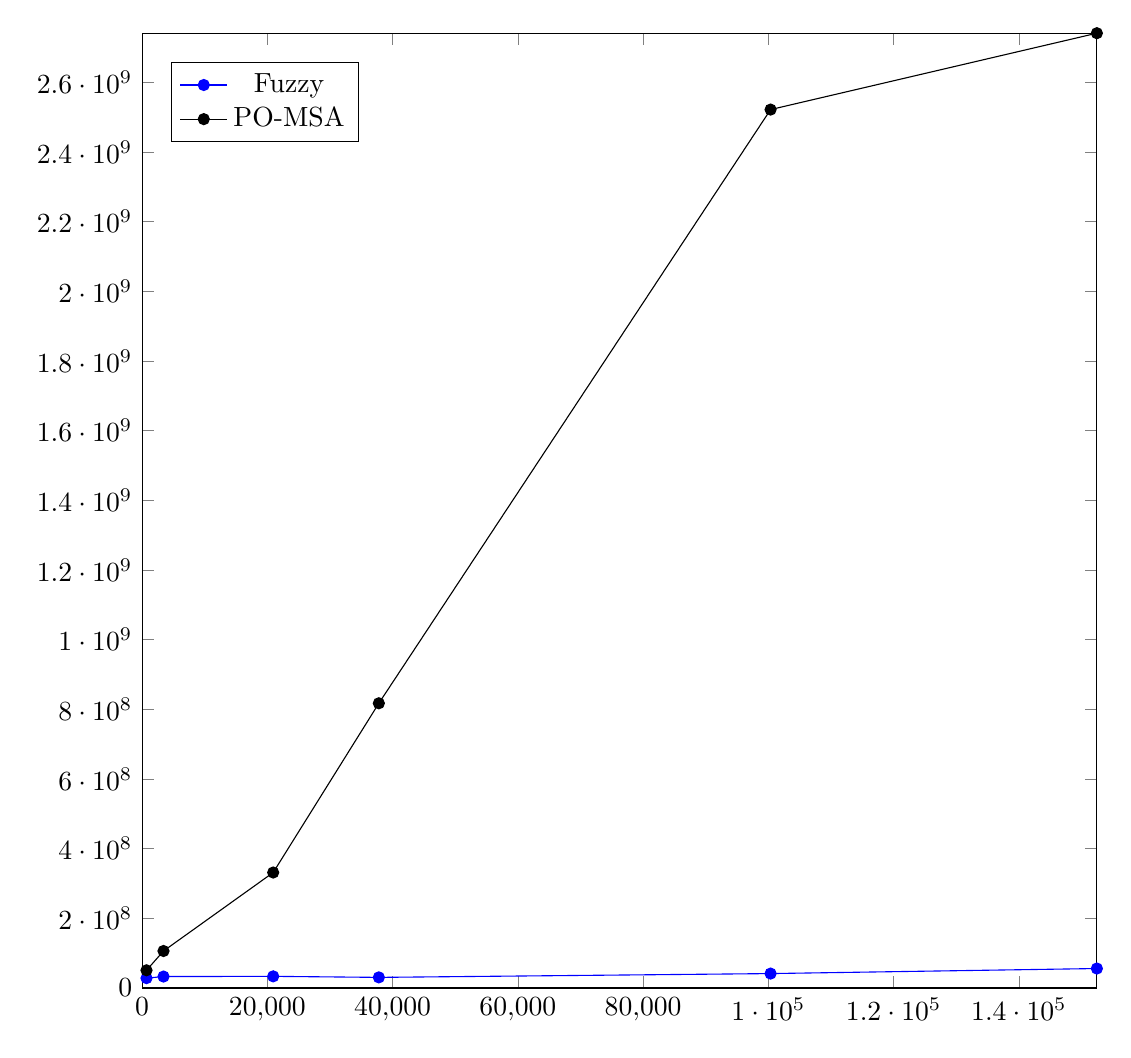
\begin{tikzpicture}
    \begin{axis}[scale only axis,height=\textwidth,width=\textwidth,xmin=0,ymin=0,xmax=152451,ymax=2741174182,scaled ticks=false, legend pos=north west]
      \addplot[color=blue,mark=*] coordinates {
        (701, 28197210)
        (3416, 32719710)
        (20931, 33308335)
        (37801,  30339892)
        (100351, 41266794)
        (152451, 55771208)
      };
      \addplot[color=black,mark=*] coordinates {
        (701, 50715055)
        (3416, 106071102)
        (20931, 331411927)
        (37801,  817322537)
        (100351, 2521874503)
        (152451, 2741174182)
      };
      \addlegendentry{Fuzzy}
      \addlegendentry{PO-MSA}
    \end{axis}
  \end{tikzpicture}
  \caption{Runtime of the alignment process as a function of the number of vertices}
  \label{fig:runtime_po-msa_fuzzy_0_0}
\end{figure}
\subsubsection{Runtime as a function of |G|}
\subsubsection{Runtime as a function of |s|}
\subsubsection{Runtime as a function of $\lambda$}
\end{document}